\documentclass[a4paper, openany, 12pt]{article}

%% подключаем стандарт библиографии
\bibliographystyle{gost71u}

%% для "Abstract" в классе book
% \newenvironment{abstract}{}{}
% \usepackage{abstract}

%% подключаем преамбулу: в ней содержится подключение всех необходимых пакетов
%% Работа с русским языком
\usepackage{cmap}			 % поиск в PDF
\usepackage{mathtext} 		 % русские буквы в формулах
\usepackage[T2A]{fontenc}	 % кодировка
\usepackage[utf8]{inputenc}	 % кодировка исходного текста
\usepackage[russian]{babel}	 % локализация и переносы

%% Пакеты для работы с математикой
\usepackage{amsmath,amsfonts,amssymb,amsthm,mathtools}
\usepackage{icomma}

%% Нумерация формул (опционально)
%\mathtoolsset{showonlyrefs=true} % показывать номера только у тех формул, на которые есть \eqref{} в тексте.
%\usepackage{leqno}               % нумерация формул слева

%% Шрифты
\usepackage{euscript}	 % шрифт "Евклид"
\usepackage{mathrsfs}    % красивый мат. шрифт

%% Некоторые полезные макросы для дебага (в случае недоверия авторам шаблона)
\makeatletter
\newcommand\thefontsize{The current font size is: \f@size pt} % пример: \section{\thefontsize}
\makeatother

%% Настройка размеров шрифтов
\makeatletter
\renewcommand\Huge{\@setfontsize\Huge{14pt}{10}}
\renewcommand\huge{\@setfontsize\huge{14pt}{21}}
\renewcommand\Large{\@setfontsize\Large{14pt}{21pt}}
\renewcommand\large{\@setfontsize\large{12pt}{10}}
\makeatother

%% Поля (геометрия страницы)
\usepackage[left=3cm,right=1.5cm,top=2cm,bottom=2cm,bindingoffset=0cm]{geometry}

%% Русские списки
\usepackage{enumitem}
\makeatletter
\AddEnumerateCounter{\asbuk}{\russian@alph}{щ}
\makeatother

%% Работа с картинками
\usepackage[font=huge]{caption}
\captionsetup{justification=centering} % центрирование подписей к картинкам
\usepackage{graphicx}                  % вставки рисунков
\graphicspath{{images/}{images2/}}     % папки с картинками
\setlength\fboxsep{3pt}                % отступ рамки \fbox{} от рисунка
\setlength\fboxrule{1pt}               % толщина линий рамки \fbox{}
\usepackage{wrapfig}                   % обтекание рисунков и таблиц текстом

%% Работа с таблицами
\usepackage{array,tabularx,tabulary,booktabs} % дополнительная работа с таблицами
\usepackage{longtable}                        % длинные таблицы
\usepackage{multirow}                         % слияние строк в таблице

%% Красная строка
\setlength{\parindent}{2em}

%% Интервалы
\linespread{1}
\usepackage{multirow}

%% TikZ
\usepackage{tikz}
\usetikzlibrary{graphs,graphs.standard}

%% Верхний колонтитул
\usepackage{fancyhdr}
\pagestyle{fancy}

%% Перенос знаков в формулах (по Львовскому)
\newcommand*{\hm}[1]{#1\nobreak\discretionary{}{\hbox{$\mathsurround=0pt #1$}}{}}

%% Дополнительно
\usepackage{float}   % добавляет возможность работы с командой [H] которая улучшает расположение на странице
\usepackage{gensymb} % красивые градусы
\usepackage{caption} % пакет для подписей к рисункам, в частности, для работы caption*
\usepackage{listings} % пакет для листингов с кодом
\lstset{              % настройки для лисингов с кодом
basicstyle=\ttfamily,
columns=flexible,
breaklines=true,
captionpos=b
}
\usepackage[font=huge]{subcaption}

% Hyperref (для ссылок внутри  pdf)
\usepackage[unicode, pdftex]{hyperref}

% Отступ перед первым абзацем в каждом разделе
\usepackage{indentfirst}

\usepackage{sectsty}
\sectionfont{\fontsize{16}{21}\selectfont}
\subsectionfont{\fontsize{14}{21}\selectfont}
\subsubsectionfont{\fontsize{14}{21}\selectfont}
\paragraphfont{\fontsize{14}{21}\selectfont}


\begin{document}
    %% титульник
    \begin{center}
    %% *название института*
    \large\textbf{Министерство образования и науки Российской Федерации \\
    Московский физико-технический институт (государственный
    университет)} \\
    \vspace{1cm}

    %% *факультет/физтех-школа*
    Физтех-школа радиотехники и компьютерных технологий \\

    %% *название базовой кафедры и лаборатории*
    %% в случае ненадобности можно удалить
    Кафедра системного программирования ИСП РАН \\
    Лаборатория (laboratory name)\\

    \vspace{3em}

    Выпускная квалификационная работа бакалавра
\end{center}

\begin{center}
    \vspace{\fill}
    %% *название вашей работы*
    \LARGE{Разработка компилятора нейронных сетей на основе инфраструктуры MLIR для процессора с матричной архитектурой}

    \vspace{\fill}
\end{center}


\begin{flushright}
    \textbf{Автор:} \\
    Студент Б01-009 группы \\
    Вязовцев Андрей Викторович \\
    \vspace{2em}
    \textbf{Научный руководитель:} \\
    *научная степень* \\
    Денисов Денис Денисович \\
    \vspace{2em}
    \textbf{Научный консультант:} \\
    *научная степень* \\
    Сергеев Сергей Сергеевич \\
\end{flushright}

\vspace{7em}

\begin{center}
    %% *лого*
    \includegraphics[width=100 pt]{MIPT_logo.jpg}\\
    Москва \the\year{}
\end{center}

%% выключаем отображение номера для этой страницы (титульник)
\thispagestyle{empty}

\newpage
\setcounter{page}{2}
\fancyfoot[c]{\thepage}
%% *надпись над верхним колонтинулом*
%% в случае ненадобности можно удалить
\fancyhead[L]{Разработка компилятора нейронных сетей на основе инфраструктуры MLIR для процессора с матричной архитектурой}
\fancyhead[R]{}
    %% аннотоция
    \begin{abstract}

    \begin{center}
        \large{Разработка компилятора нейронных сетей на основе инфраструктуры MLIR для процессора с матричной архитектурой} \\
    \large\textit{Вязовцев Андрей Викторович} \\[1 cm]

    Краткое описание задачи и основных результатов, мотивирующее прочитать весь текст.

    \vfill

    \textbf{Abstract} \\[1 cm]

    FIXME: English abstract? 
    \end{center}

\end{abstract}
\newpage
    %% содержание
    \tableofcontents{}
    \newpage

    \section{Введение}
\label{sec:Chapter0} \index{Chapter0}

Нейронные сети в последниее время испытывают большой подъём.
Это происходит, прежде всего, благодаря успехам Chat GPT,
которая показала новые возможность для обработки естественной речи.
Стоит отметить, что развитие этой сферы происходит не только за счёт
совершенствования точности ответов нейронных сетей. Например,
разбатываются процессоры с матричной архитектурой, которые могут
быть встроены в смартфоны. Очевидно, что такие решения будут
востребованы на мобильном рынке, который занимает крупную часть
всего IT-рынка.

Для использования таких процессоров необходим широкий набор утилит,
в том числе и компиляторы. Основной задачей любого компилятора
является получение наиболее оптимального с точки зрения
производительности машинного кода при сохранении всех свойств
исходной программы. Заметим, что в таких компиляторах помимо
традиционных техник оптимизации, таких как удаление мёртвого кода,
распостранения констант, сокращения общих подвыражений и других,
должны применяться другие техники, связанные с математическими
свойствами тензоров и спецификой целевой архитектуры.

В силу описанных выше причин идут активные исследования в
области компиляторов для нейронных сетей, в том числе и нашей
лабораторией. В данной работе будет исследованы особенности
целевой архитектуры и представлены способы генерации эффективого
машинного кода. 

\newpage

    \section{Постановка задачи}
\label{sec:Chapter1} \index{Chapter1}

Задача исследования: разработать компилятор нейронных сетей для процессоров
Ascend, основанных на архитектруре DaVinci, с использованием инфраструктуры
LLVM MLIR и обеспечить генерацию эффективного машинного кода в нём.
Для достижения данной задачи были поставлены следующие цели исследования:

\begin{enumerate}
    \item Исследовать архитектуру современных популярных нейронных сетей
          и типичные для них операции.
    \item Исследовать подходы к эффективному исполнению нейронных сетей,
          в том числе использование специальных процессоров (NPU),
          компиляторов с разными целевыми архитектурами (CPU, GPU, NPU),
          узнать их особенности и используемые в них оптимизации.
    \item Изучить инфраструктуру LLVM MLIR и предоставляемые ею возможности
          для написания собственного компилятора.
    \item Исследовать архитектуру DaVinci, принцип работы нейроматричного
          процессора и её язык ассемблера.
    \item Разработать набор операторов для целевой архитектуры DaVinci в
          инфраструктуре MLIR.
    \item Исследовать и предложить методы генерации оптимального машинного
          кода для некоторых типичных операций нейронных сетей.
    \item Реализовать наиболее эффективные способы генерации машинного кода,
          исследовать их производительность.
\end{enumerate}

\newpage

    \section{Обзор современных нейронных сетей}
\label{sec:Chapter2} \index{Chapter2}

\subsection{Общие соображения}

Искуственная нейронная сеть --- математическая модель, а также её программное или
аппаратное воплощение, построенная по принципу организации биологических нейронных
сетей --- сетей нервных клеток живого организма. Этот принцип отражается в её
устройстве: нейронная сеть состоит из некольких слоёв, каждый из которых принимает
информацию с предыдущего, обрабатывает её каким-то образом, а  затем передаёт её
на следующий слой.

Благодаря новым исследованиям в этой области, нейронные сети нашли большое
количество применений в разных сферах жизни. В медицине они позволяют проводить
более точную диагностику заболеваний (например, онкологии), создавать портативные
устройтва для диагностики (например, для проведения ЭКГ). Они используются
для обработки больших данных в разных исследовательских областях, таких как
астрономия и геологоразведка. Также они упрощают жизнь в робототехнике и
автоматизации производства.

Рассмотрим наиболее популярные архитектуры нейронных сетей, их основные особенности.

\subsection{Обработка естественного языка}

Обработка естественного языка --- общее направление искусственного интеллекта и
математической лингвистики. Оно изучает проблемы компьютерного анализа и синтеза
текстов на естественных языках. Применительно к искусственному интеллекту анализ
означает понимание языка, а синтез --- генерацию грамотного текста. Одним из
подходов к решению данной задачи стала архитектура трансформер, представленная
компанией Google в 2017 году. Эта архитектура используется в переводчиках
(например, от компаний Яндекс и Google) и в чат-ботах (например, Chat GPT).
BERT, GPT-3, LLaMA --- модели, основывающиеся на архитектуре трансформер.

Многие из таких моделей можно скачать, после чего изучить их внутреннее
устройство. Нами была выбрана модель BERT. Не погружаясь в детали реализации
можно заметить, что подавляющее большиство операций в ней занимают
умножения матриц. По этой причине эта операция была выбрана для
дальнейшего исследования.

\subsection{Компьютерное зрение}

Компьютерное зрение --- теория и технология создания машин, которые могут
производить обнаружение, отслеживание и классификацию объектов. Распознавание
изображений может быть полезно в любой сфере, например, в сельском хозяйстве ---
для обнаружения болезни растений, в области безопасности --- для обнаружения
преступников и т.д.

Одно из наиболее популярных решений в этой области --- свёрточные нейронные
сети. Принцип их работы схож с работой зрительной коры головного мозга.
Основываются они на операции свёртки (конволюции). В функциональном анализе
она применяется к двум функциям и возвращает третью, соответствующую их
взаимной корреляции. Проще говоря, их можно интерпретировать как <<схожесть>>
двух функций.

В нейронных сетях свёртка применяется к изображениям, её схему можно увидеть
ниже. На часть изображения <<накладывается>> ядро, т.е. эта часть скалярно
умножается на ядро. Получившийся результат является каким-то признаком, он
записывается в результирующую матрицу --- матрицу выходных признаков
(output feature map). Стоит отметить, что общий случай свёркти несколько
сложнее, более подробно этот вопрос будет рассмотрен в соответствующей
главе.

\begin{figure}[h!]
    \centering
    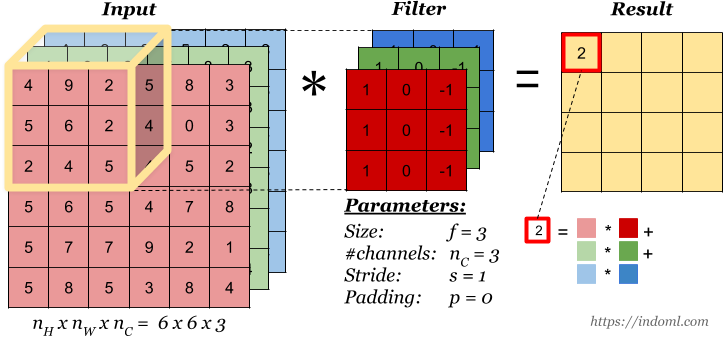
\includegraphics[scale=0.5]{Convolution.png}
    \caption{Операция свёркти для изображения с тремя цветами}
\end{figure}

Существует большое количество свёрточных нейронных сетей: LeNet-5, AlexNet,
VGG, GoogLeNet, ResNet, Inception. Нами была выбрана ResNet для дальнейшего
исследования. Она представлена несколькими вариантами, которые отличаются
количеством слоёв, а следовательно, точностью вычислений и размерами весов
модели. Модель с 18 слоями представлена на рисунке ниже. Как видно из
рисунка, в ней используются только операции свёркти. Но внутри них также
есть операции сложения и $Relu$, где

\[
    Relu(x) =
        \begin{cases*}
            x, ~ x \geqslant 0 \\
            0, ~ x < 0
        \end{cases*}
\]

\begin{figure}[h!]
    \centering
    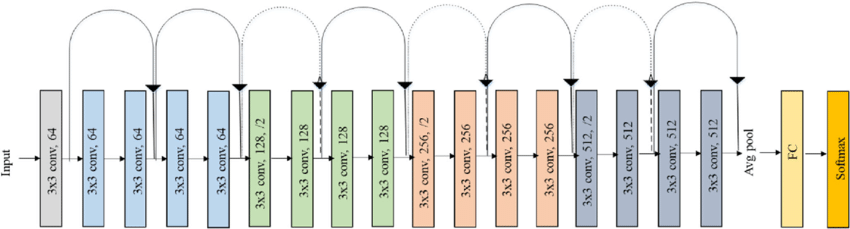
\includegraphics[scale=0.5]{ResNet18.png}
    \caption{Модель ResNet18}
\end{figure}

\newpage

    \section{Умножение матриц и свёртка с точки зрения процессора и компилятора}
\label{sec:Chapter3} \index{Chapter3}

\subsection{Свёртка}

Реализация свёртки на нейроматрицных процессоров несколько сложнее, чем умножения.
На некоторых архитектурах (FIXME: ссылка) она поддержана нативно. К сожалению, наша
не является таковой. Но с помощью особого преобразования её можно свести к 
умножению матриц. Приведём некоторые общие соображения, которые позволят понять его.

Итак, пусть есть входное изображение (\textit{image}) размеров $H_i \times W_i$,
содержащее $C$ цветов. Будем называть его \textit{входной картой признаков}
(\textit{input feature map}). Ядро (\textit{kernel}) свёртки представляет из
себя небольшую матрицу размеров $H_k \times W_k$ (характерный размер --- $3-5$).
Ядро имеет такое же количество входных цветов $C$, но также имеет и $F$
выходных цветов. Таким образом, изображение имеет формат $H_i W_i C$,
а ядро --- $F H_k W_k C$. Выходная карта признаков, имеет структуру, схожую
со входной: $H_o W_o F$, где $H_o = H_i - H_k + 1$, $W_o = W_i - W_k + 1$
в простейшем случае. Если обозначить: $a$ --- входная карта, $k$ --- ядро,
$c$ --- выходная, то свёрка выражается следующей формулой:

\[
    c_{ijf} = \sum \limits_{h = 0}^{H_k} \sum \limits_{w = 0}^{W_k}
              \sum \limits_{c = 0}^{C} a_{i+h, j+w, c} \cdot k_{f h w c}
\]

Заметим, что операция чем-то схожа на скалярное умножение векторов
(если цвета считать вектором) или матричное умножение. Если первый тензор
преобразовать в матрицу $A$, где одной строке будет соответвовать одна
такая сумма (т.е. размеры матрицы станут $H_o W_o \times H_k W_k C$), а
ядро --- в матрицу $K$ размеров $H_k W_k C \times F$, то выходная
матрица $C = A \times K$. Этот процесс преобразования входной карты
признаков называется \textit{img2col} (\textit{image-to-column}),
оно содержится в архитектуре команд целевого процессора.

Таким образом, свёрка есть композиция \textit{img2col} и умножения матриц.
Отметим, что в реальности свёртка имеет такие параметры, как
\textit{stride}, \textit{dilation} и \textit{pad}. Они усложняют
приведённые формулы, но не меняют сути происходящего. Также в
качестве обобщения можно взять $N$ изображений, форматы входной и
выходной карт приобретают вид $N H_i W_i C$ и $N H_o W_o F$ соответственно.

\newpage

    \section{Обзор существующих компиляторов нейронных сетей}
\label{sec:Chapter4} \index{Chapter4}

\subsection{Инфраструктуры и стандарты}

Для удобного проектирования, обучения и запуска нейронных сетей создаются
фреймворки (т.~е. библиотеки), поддерживающие большое количество операций
нейросетей и содержащие некоторые заранее натренированные модели и открытые
датасеты (наборы данных), использованные для их обучения. Наиболее популярными
из таких являются \textit{PyTorch} и \textit{TensorFlow}. Обучение и исполнение
моделей в этих фреймворках возможно как на CPU, так и на GPU.

Очевидно, что PyTorch и TensorFlow являются не единственными в своём роде.
По этой причине добавление возможностей исполнения на специализированном
процессоре в каждый фреймворк является нерациональным. Для унификации работы
с фреймворками, создаются стандарты, такие как \textit{ONNX}, \textit{TOSA}
или \textit{StableHLO}. Они создают единую точку входа для специализированных
компиляторов: сначала модель из любого фреймворка конвертируется в модель на
языке стандарта, и именно эту модель принимает на вход компилятор для создания
архитектурно-специфичного кода. Среди таких компиляторов можно выделить
\textit{XLA}, \textit{MindSpore}, \textit{ONNX runtime}. Но все они также
нацелены на исполнение на самых распростаннённых архитектурах: x86-64 (в т.~ч.
с векторизацией при помощи AVX), ARM, GPU (в т.~ч. с использованием технологий
CUDA от Nvidia и ROCm от AMD). Их использование в качестве основы для создания
компилятора для архитектуры DaVinci означало бы написание полного цикла
компиляции из стандарта до ассемблерных инструкцию практически <<с нуля>> и
не давало бы никаких преимуществ. 

\subsection{Оптимизации и полиэдральная компиляция}

Как было упомянуто ранее, одними из основных операций в нейронных сетях
являются умножения матриц и свёртки. Эти операции представляют из себя большое
количество простых и однотипных арифметических операций (сложения и умножения).
По этой причине их можно оптимизировать средствами векторизации и
переупорядочивания обхода циклов. Для этих целей была создана математическая
модель, основанная на алгебраическом представлении программ и их
преобразований, --- полиэдральная модель. В них цикл является полиэдром,
т.~е. многомерным многогранником в аффином пространстве. Аффинные преобразования
этого пространства соответствуют преобразованиям цикла, изменениям порядка
обхода элементов.

Рассмотрим некоторые проекты, использующие этот подход, а именно \textit{TVM},
\textit{Halide} и \textit{Polly}. Polly является частью проекта LLVM и
преобразует LLVM IR для генерации оптимального кода. Его использование привело
бы к необходимости добавления новых инструкций в LLVM IR и не давало бы
достаточных уровней абстракции. Инфраструктуры TVM и Halide позволяют
создавать новые операции, но требуют, чтобы для них был задан способ исполнения.
Такой подход является неудобным, т.~к. это означает, что после преобразований
код должен быть транслирован в ассемблерные инструкции по неким сложным
шаблонам. Более того, в Halide это исполнение задаётся исключительно скалярном
виде. К сожалению, единственный существующий компилятор для Ascend,
преобразующий ONNX модели, --- \textit{Automatic kernel generator (AKG)},
являющийся частью MindSpore, пошёл по этому пути и использует Halide в качестве
инфраструктуры.

\subsection{Итог}

Существует большое количество различных компиляторов для нейронных сетей. Они
используют разлиные подходы для генерации кода, но во многом повторяют друг
друга. По этой причиной одно из крупнейших сообществ --- LLVM --- решило
создать переиспользуемую инфраструктуру MLIR, собирающую в себя лучшее из
различных подходов и техник, в т.~ч. и полиэдральной компиляции. На данный
момент проект активно развивается и является самой современной крупной
инфраструктурой.

\newpage

    \section{Инфраструктура LLVM MLIR}
\label{sec:Chapter5} \index{Chapter5}

Как можно заметить из предыдущего параграфа, компиляторы из предыдущего параграфа
решали сходные задачи, но они отличались некоторыми деталями, из-за чего
приходилось создавать новый компилятор и пересоздавать большое количество
компонентов. В связи с этим сообщество разработчиков LLVM придумали и реализовали
переиспользуемую и расширяемую инфраструктуру MLIR.

Основная концепция MLIR --- диалекты. Диалект объединяет в себе типы, операции
и их преобразования на каком-либо уровне абстракции. В MLIR существует более 40
встроенных диалектов, имплентация собственных диалектов возможна с помощью
декларативного языка \textit{ODS} или на языке C++.

Рассмотрим некоторые диалекты, которые будут использованы в данной работе.

\begin{enumerate}
    \item HLO --- диалект, который позволяет представлять модели нейросетей,
          написанных на tensorflow, в представлении MLIR. Несмотря на то,
          что он не является стандартным и представлен в виде отдельного
          репозитория, пользуется популярностью благодаря широкой
          известности tensorflow.

    \item tensor --- диалект для представления тензоров и операций,
          позволяющих менять форму тензоров, изменять их размеры,
          <<вырезать>> и <<вставлять>> части из них. Стоит отметить, на
          данном уровне абстракции считается, что тензоры не имеют какого-то
          конкретного расположения в памяти. Этим они похожи на виртуальные
          регистры из теории компиляторов.

    \item memref --- диалект, который абстрагирует работу с многомерными
          массивами. Операции в этом диалекте схожи с операциями из диалекта
          tensor, но этих диалектов есть существенное отличие: memref является
          представлением реальных объектов.

    \item affine --- диалект, который предоставляет возможность работы с
          аффинными циклами и преобразованиями над ними, тем самым реализуя
          возможности для полиэдральной компиляции.

    \item scf (structured control flow) --- диалект, в котором представлен
          структурный поток исполнения (т.е. в виде системы вложенных блоков).

    \item cf (control flow) --- диалект, предсталяющий исполнение в виде графа
          потока управления.

    \item func --- диалект, реализующий концепцию функций, их вызова, передачи
          аргументов, возвращения значения.

    \item transform --- диалект, необходимый для реализации преобразований
          внутри одного диалекта. С его помощью операция предсталяется в виде
          одной или нескольких операций (зачастую, более эффективных по
          производительности, чем исходная), что позволяет подготовить код
          для дальнейшего lowering-а или оптимизировать его.

    \item llvm --- самый низкоуровневый диалект, реализующий семантику LLVM IR.
          Его можно перевести в LLVM IR непосредственно, после чего
          воспользоваться другими средствами LLVM для компиляции. Отметим, что
          получение кода именно в таком представлении является нашей
          непосредственной задачей.
\end{enumerate}

Выше были перечислены лишь те диалекты, которые непосредственно будут
использованы во время lowering-а из HLO в llvm. Помимо в них в MLIR существует
большое количество других диалектов, например, для графических ускорителей (GPU),
для векторных инструкций (AVX512), для распараллеливания исполнения программ
(OpenMP) и другие. Общая диаграмма диалектов и их соотношения представлена на
рисунке ниже.

\begin{figure}[h!]
    \centering
    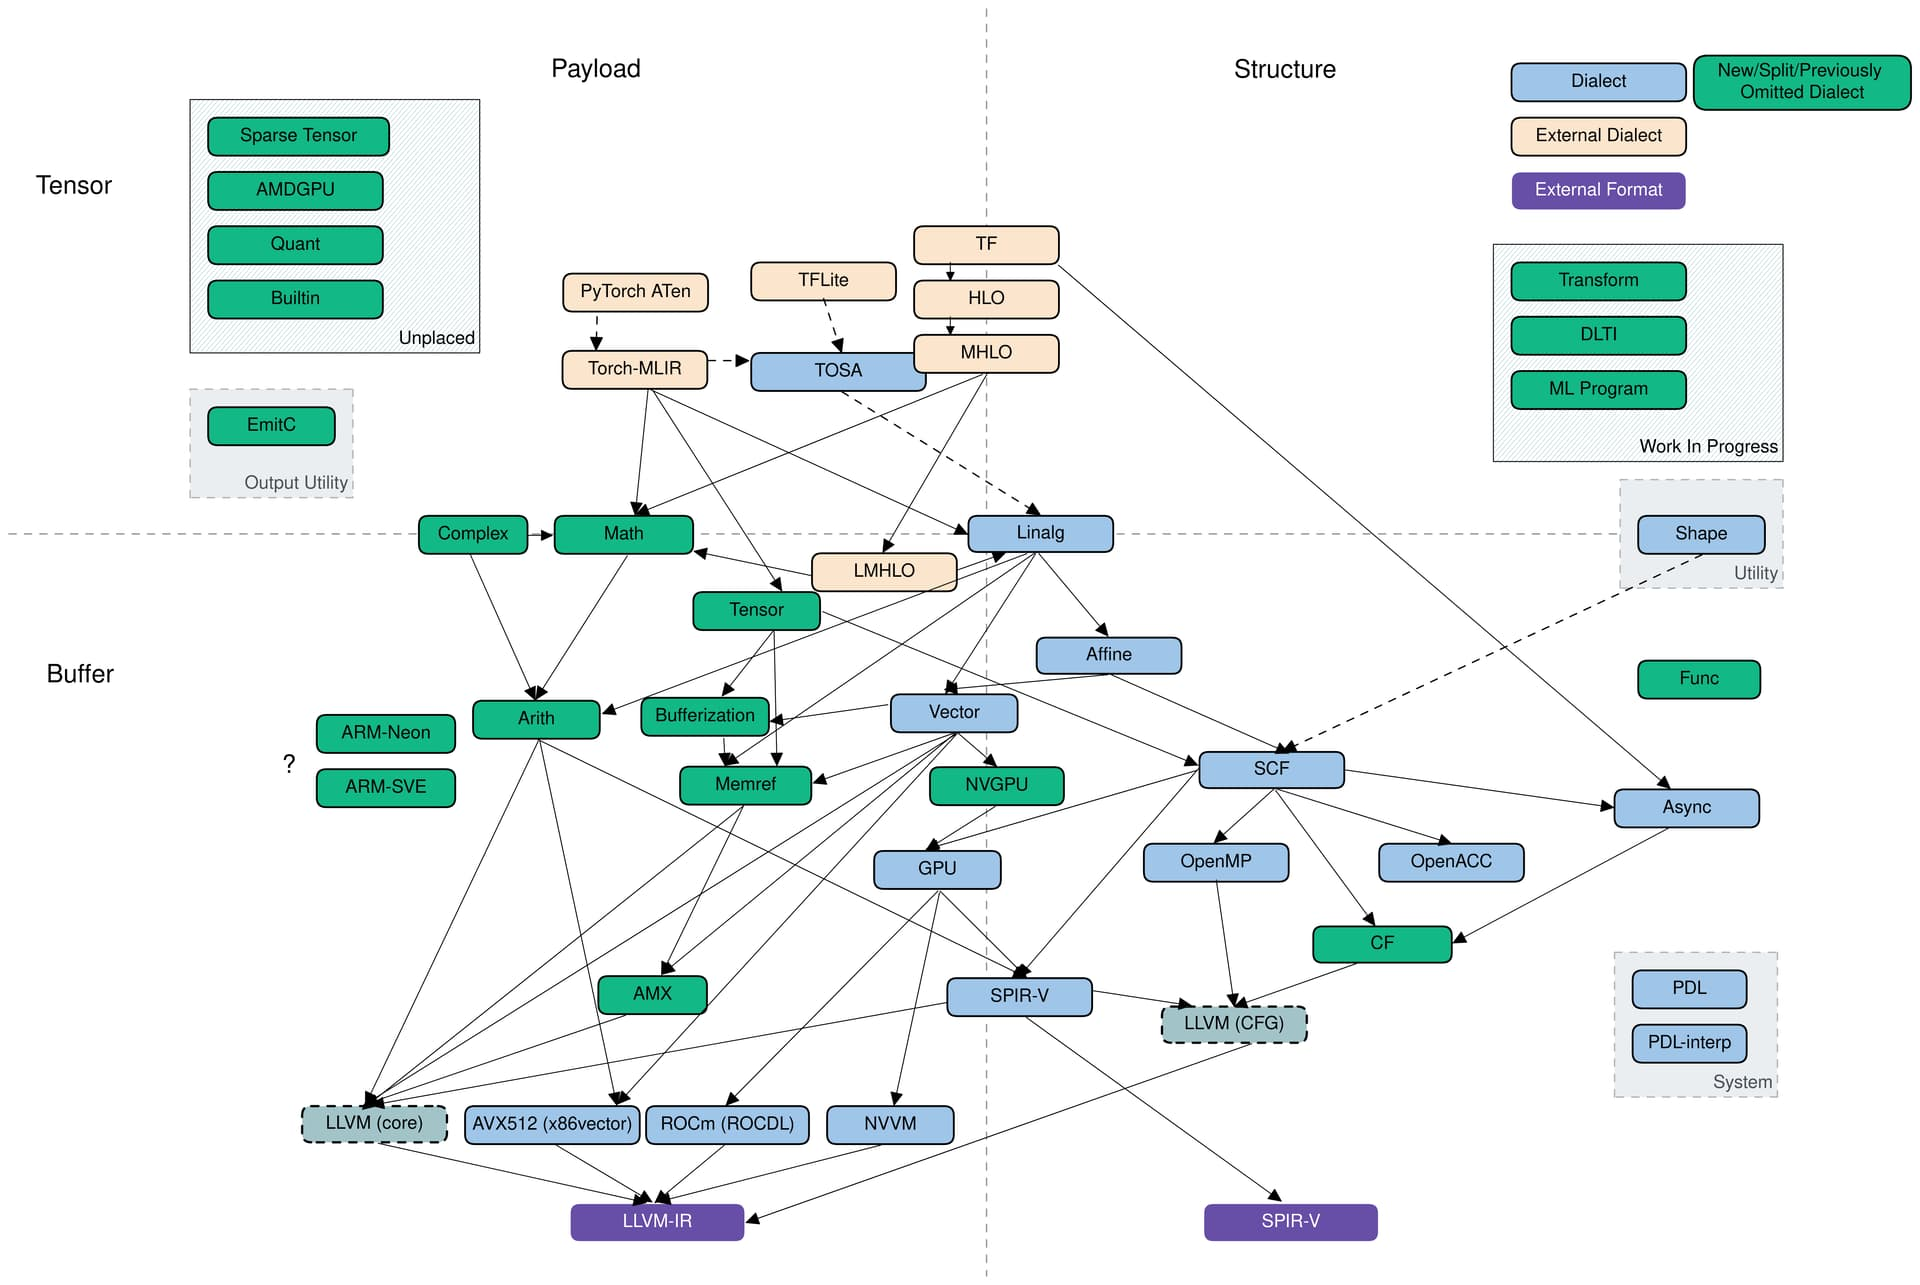
\includegraphics[scale=0.25]{MLIR_Dialects.jpg}
    \caption{Структура проекта MLIR и соотношения диалектов в них}
\end{figure}

\newpage

    \section{Обзор архитектуры DaVinci}
\label{sec:Chapter6} \index{Chapter6}

\subsubsection{Общее описание}

Архитектура DaVinci --- нейропроцессор (NPU, neural processing unit),
разработанный компаней HiSilicon (подразделение Huawei). В отличие от
обычных CPU и GPU, которые необходимы для вычислений общего назначения,
и ASIC, предназначенной для конкретного алгоритма, архитектура Da Vinci
предназначена для исполнения уже обученных нейронных сетей. Работа с NPU
является обычной схемой гетерогенных вычислений, в ней CPU является хостом
(главным устройством, которое запрашивает вычисления), а NPU --- девайсом
(подчинённым устройством, производящим вычиления). Взаимодействие между ними
происходят по следующему алгоритму:

\begin{enumerate}
    \item Хост производит инициализацию, необходимую для общения с девайсом.
    \item Хост аллоцирует память (общую для него и девайса) и загружает данные в неё.
    \item Хост загружает объектный файл девайса и регистрирует функцию для исполнения.
    \item Хост передаёт указатели на аллоцированную память и даёт команду к исполнению.
    \item Девайс исполняет выбранную функцию.
    \item Хост копирует результат исполнения девайса к себе.
\end{enumerate}

Процессоры, основанные на архитектуре DaVinci и их основные характеристики
представлены в таблице ниже:

\begin{table}[h!]
    \centering
    \begin{tabular}{|c|c|c|c|c|}
        \hline
        Процессор & Производительность для float 16/int 8 & Мощность & Тех. процесс  \\ \hline
        Ascend 910 & 320/640~терафлопс & 310~Вт & 7~нм, N7+ \\ \hline
        Ascend 310 & 16/8~терафлопс & 8~Вт & 12~нм, FFC \\ \hline
    \end{tabular}
\end{table}

Теперь перейдём к внутреннему устройствую чипа Ascend. Схема архитектуры
представлена на рисунке. Рассмотрим её основные особенности.

\begin{figure}[h!]
    \centering
    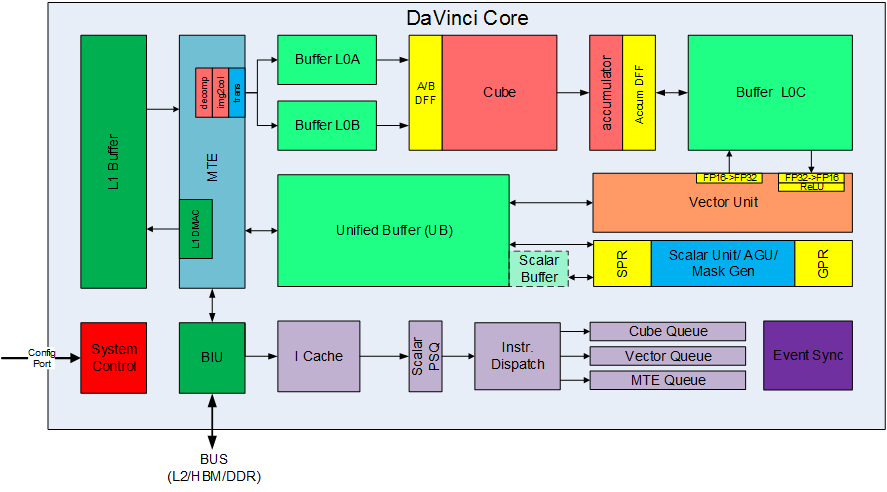
\includegraphics[scale=0.5]{DaVinci.png}
    \caption{Архитектура DaVinci}
\end{figure}

В ядре есть три вычислительных юнита: матричный, векторный и скалярный,
которые используются для соответствующих вычилений.  Исполнение на юнитах
происходит параллельно, для каждого юнита существует
отдельная, независимая очередь задач. Ещё три очереди предназначены для
копирования из разных буфферов друг в друга (о них речь пойдёт ниже).
Для синхронизации очередей используются команды \texttt{set\_flag} и \texttt{wait\_flag},
которые по своей сути представляют систему событий. Первая команда сигнализирует,
что событие произошло, а вторая запускает ожидание события. Правильное
использование механизмов синхронизации позволяет значительно увеличить
загрузку всех юнитов и, следовательно, снизить общее время исполнения.
В данной работе не будут рассматривать проблемы с расстановкой операций
синхронизации и будет считаться, что они всегда расставлены наиболее
оптимальным образом.

\subsubsection{Матричный юнит}

Матричный юнит на вход принимает матрицы с типом элементов \texttt{float 16}
или \texttt{int 8}, на выходе же элементы имеют тип \texttt{float 16},
\texttt{float 32} или \texttt{int 32}. Умножение работает в двух режимах:

\begin{enumerate}
    \item Обычное умножение: $C = A \times B$
    \item Режим накопления: $C = A \times B + C$, т.~е. результат текущего
          умножения прибавляется к предыдущему.
\end{enumerate}

Каждая из входных матриц должна быть разбита на блоки $16 \times 16$
(в случае \texttt{float 16}) или $16 \times 32$ (в случае \texttt{int 8}).
Расположение элементов внутри блоков и блоков относительно друг друга также
различно. Существуют две стратегии размещения: про строкам (формат \texttt{Z})
и по столбцам (формат \texttt{N}). Примем обозначение: размещение внутри блока
обозначается строчной буквой, а между блоками --- заглавной. При умножении
матрица $A$ должна быть заранее быть записана в формате \texttt{Zz},
матрица $B$ --- в формате \texttt{Zn}, а выходная матрица $C$ будет \texttt{Nz}.

Матричный юнит работает по принципу систолического массива.
Систолический массив --- однородная сеть тесно связанных блоков обработки данных.
Его схему для архитектуры DaVinci можно увидеть на картинке ниже.

Принцип умножения довольно прост: за первый такт (FIXME: лучше не использовать
слово такт в данном контексте) происходят все умножения,
после чего за оставшиеся четыре такта произведения суммируются. Таким
образом, за пять тактов можно перемножить две матрицы \texttt{16x16}.
Матричный юнит, итерируясь по матрицам и перемножая их поблочно, быстро
получает результат перемножения.

\begin{figure}[h!]
    \centering
    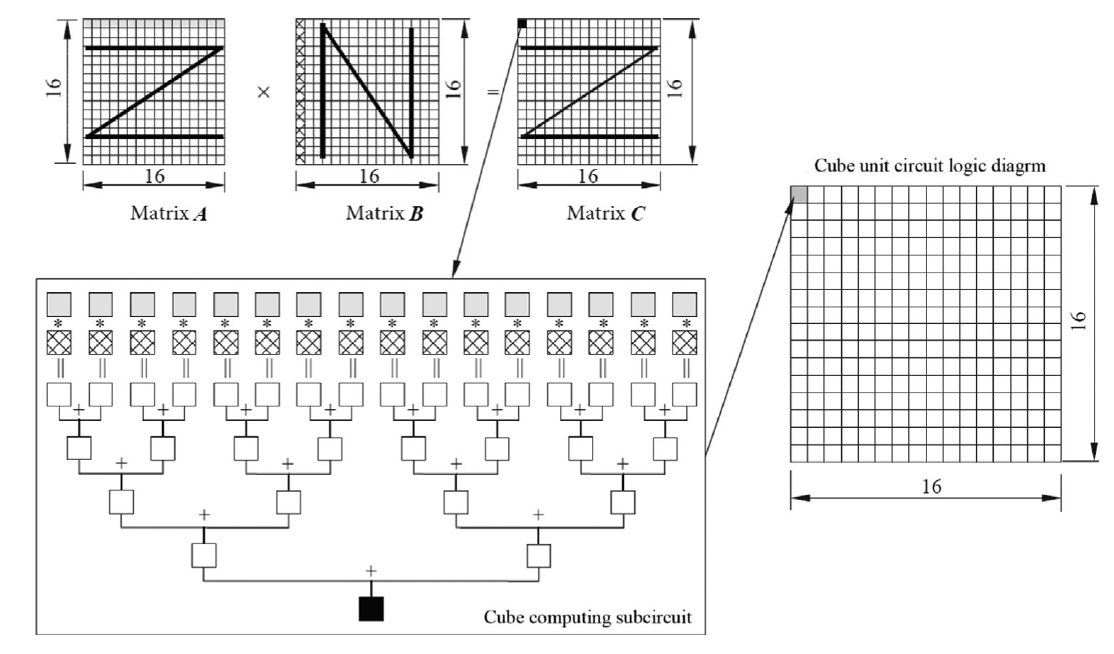
\includegraphics[scale=0.5]{Systolic.png}
    \caption{Схема вычисления в матричном юните}
\end{figure}

\subsubsection{Векторный юнит}

Теперь рассмотрим работу векторного юнита. Существуют два режима работы:
\textit{common} и \textit{VA}. В обоих случаях память делится на блоки
по 32 байта, а векторная операция представляется в виде цикла, на каждой
итерации которого обрабатывается 8 блоков. Таким образом, за одну итерацию
может быть обработано 128 элементов типа \texttt{float 16} или 64 элемента
32-разрядных типов (\texttt{float 32}, \texttt{int 32}). Стоит отметить, что
не обязательно обрабатывать такое количество элементов. Для выбора, с какими
именно элементами будет работать операция необходимо задать маску. Векторный
юнит обрабатывает только те элементы, на позиции которых в маске стоит бит 1.
На каждой следующей итерации блоки сдигаются на заранее заданный шаг,
после чего операция повторяется. Отличаются режимы способом описания этих блоков.
В случае \textit{VA} режима блоки задаются в виде восьми указатей, а в случае
\textit{common} --- указателем на первый блок и шагом между блоками. Для первого,
второго аргумента и результата шаг может быть различным. 
Юнит поддерживает большое количество операций: математических, логических,
приведения типов и т.~д. Есть и спецефичные операции: \textit{relu}, часто
используемый в нейронных сетях, операция транспонирования.

\subsubsection{Память}

Память ядра неоднородна. В ядре существует 5 буферов:
L1, L0A, L0B, L0C, UB. Также существует внешняя память (GM), через которую
происходит общение с хостом. Опишем общую схему потока данных между этими кэшами.
Данные из внешней памяти загружаются в L1 и UB. Данные в UB предназначены для
обработки векторным и скалярным юнитами. Данные из L1 загружаются в L0A и L0B,
которые соответствуют матрицам A и B матричного умножения. Результат после
перемножения (которое, как было упомянуто раньше, выполняется матричным юнитом),
попадает в буфер L0C, из которого происходит данные отправляются в UB. Выгрузка
результата вычислений во внешнюю память возможна только из UB. Отметим, что
описанные выше буферы имеют небольшой размер, что является одной из основных
проблематик нашей работы. Более подробно этот вопрос будет рассмотрен в главе,
посвященной ловерингу.

\subsubsection{Свёртка}

Реализация свёртки на нейроматрицных процессоров несколько сложнее, чем умножения.
На некоторых архитектурах (FIXME: ссылка) она поддержана нативно. К сожалению, наша
не является таковой. Но с помощью особого преобразования её можно свести к 
умножению матриц. Приведём некоторые общие соображения, которые позволят понять его.

Итак, пусть есть входное изображение (\textit{image}) размеров $H_i \times W_i$,
содержащее $C$ цветов. Будем называть его \textit{входной картой признаков}
(\textit{input feature map}). Ядро (\textit{kernel}) свёртки представляет из
себя небольшую матрицу размеров $H_k \times W_k$ (характерный размер --- $3-5$).
Ядро имеет такое же количество входных цветов $C$, но также имеет и $F$
выходных цветов. Таким образом, изображение имеет формат $H_i W_i C$,
а ядро --- $F H_k W_k C$. Выходная карта признаков, имеет структуру, схожую
со входной: $H_o W_o F$, где $H_o = H_i - H_k + 1$, $W_o = W_i - W_k + 1$
в простейшем случае. Если обозначить: $a$ --- входная карта, $k$ --- ядро,
$c$ --- выходная, то свёрка выражается следующей формулой:

\[
    c_{ijf} = \sum \limits_{h = 0}^{H_k} \sum \limits_{w = 0}^{W_k}
              \sum \limits_{c = 0}^{C} a_{i+h, j+w, c} \cdot k_{f h w c}
\]

Заметим, что операция чем-то схожа на скалярное умножение векторов
(если цвета считать вектором) или матричное умножение. Если первый тензор
преобразовать в матрицу $A$, где одной строке будет соответвовать одна
такая сумма (т.е. размеры матрицы станут $H_o W_o \times H_k W_k C$), а
ядро --- в матрицу $K$ размеров $H_k W_k C \times F$, то выходная
матрица $C = A \times K$. Этот процесс преобразования входной карты
признаков называется \textit{img2col} (\textit{image-to-column}),
оно содержится в архитектуре команд целевого процессора.

Таким образом, свёрка есть композиция \textit{img2col} и умножения матриц.
Отметим, что в реальности свёртка имеет такие параметры, как
\textit{stride}, \textit{dilation} и \textit{pad}. Они усложняют
приведённые формулы, но не меняют сути происходящего. Также в
качестве обобщения можно взять $N$ изображений, форматы входной и
выходной карт приобретают вид $N H_i W_i C$ и $N H_o W_o F$ соответственно.


\newpage

    \section{Заключение}
\label{sec:Chapter5} \index{Chapter5}

Здесь надо перечислить все результаты, полученные в ходе работы. Из текста
должно быть понятно, в какой мере решена поставленная задача.

\newpage

    \section{Lowering операций и возможные стратегии}
\label{sec:Chapter8} \index{Chapter8}

Изучив особенности целевой архитектуры, можно перейти к рассмотрению
конкретных стратегий lowering-а и их классификации. В связи с тем, что именно
работа с внешней память занимает большую часть времени, будем пытаться
оптимизировать еë. Как было упомянуто в одной из предыдущих глав, из-за малого
объëма внутренних кэшей данные приходится загружать частями, при этом каждая часть,
скорее всего, будет загружена несколько раз. В связи с этим, уменьшение количества
повторных загрузок --- самый простой способ оптимизации, а стратегия разбиения,
при которой достигается наименьшее количество повторных загрузок, будет считаться
нами наиболее оптимальной.

\newpage

    \section{Заключение}
\label{sec:Chapter5} \index{Chapter5}

Здесь надо перечислить все результаты, полученные в ходе работы. Из текста
должно быть понятно, в какой мере решена поставленная задача.

\newpage

    \section{Результаты}
\label{sec:Chapter10} \index{Chapter10}

WIP

Output Stationary --- самая эффективная стратегия? Графики (или в аппендикс?)? 

\newpage

    \section{Заключение и дальнейшая работа}
\label{sec:Chapter11} \index{Chapter11}

WIP

Работа не закончена...

\newpage


    %% НЕ ТРОГАЙТЕ!!!
    \nocite{*}
    \bibliography{references}

    %% в зависимости от надобности подключаем раздел "Приложение"
    % \newpage
    % \input{Appendix.tex}
\end{document}
